\chapter{Implementazione}
\label{implementazione}

In questo capitolo spiegheremo in dettaglio l'implementazione delle componenti del progetto. Cominceremo con un'analisi del Interprete del SoftCore e di tutte le sue componenti, per poi spiegare i cambiamenti richiesti per far funzionare il codice dentro un kernel compilabile per una FPGA. Successivamente descriveremo in dettaglio l'interfaccia lato host, e come si svolge il processo di compilazione del progetto. Esploreremo una versione dell'interprete con i registri in virgola Mobile (floating-point).
Verrà analizzato come l'interfaccia host cambia con l'istanziazione di più Control Unit.
Si conclude con una analisi della versione dell'interprete progettata per emulare una GPU senza controllore SIMD.

\clearpage

\section{Interprete Softcore}
\label{Interprete Softcore}
In questa sezione, esploreremo le componenti dell'interprete.
È necessario sottolineare che questa è la versione progettata per la compilazione ed esecuzione su una qualsiasi macchina host e scritta interamente nel linguaggio C, le modifiche necessarie per l'esecuzione sulla FPGA saranno dettagliate nella prossima sezione \ref{Interprete Kernel}.

\vspace{0.5cm}

\noindent Il codice completo relativo alla sezione seguente è presente nell'appendice (ref a cpu.c e cpu.h)

\vspace{0.5cm}

Per lo sviluppo di questo interprete è stata seguita la documentazione ufficiale del Softcore Microblaze \cite{sitoMicroblaze}.

\vspace{0.5cm}

Nonostante questo interprete non replichi il funzionamento hardware effettivo del processore Microblaze, comunque rispetta il fondamentale paradigma di qualsiasi processore. Questo si basa sull'utilizzo di registri per mantenere lo stato della CPU e portare avanti la computazione e su l'uso di una memoria per immagazzinare e recuperare i dati.

È importante evidenziare che nella implementazione seguente si è optato per l'utilizzo di bit field per le strutture dati, cosi da migliorare la chiarezza e leggibilità delle dimensioni dei singoli campi, mantenendo al fedeltà alla documentazione. 

\vspace{0.6cm}

\noindent \textbf{Registri:}

\vspace{0.2cm}

\noindent Cominciamo illustrando la struttura dei registri, partendo dalla loro implementazione:
\begin{lstlisting}[language=C]
struct Registers
{
    int32_t r[32];
    int16_t im;
    bool c : 1;
    int32_t pc;
};
\end{lstlisting}
\label{structreg}

\noindent Come è possibile vedere dalla implementazione, il processore dell'interprete è dotato dei seguenti registri: 
\begin{itemize}
    \item \texttt{r}: un array da $32$ registri interi a \texttt{32 bit}.
    \item \texttt{im}: ovvero un registro da \texttt{16 bit} il quale viene usato dalla istruzione \texttt{imm} (\ref{imm}) per estendere l'immediato precedentemente istanziato da \texttt{16} a \texttt{32 bit}.
    \item \texttt{c}: ovvero una flag da \texttt{1 bit} il quale segnala il caso in cui l'istruzione precedente ha generato un overflow. 
    \item \texttt{pc}: Program Counter, un registro che indica la prossima istruzione da eseguire.
\end{itemize}    

\noindent \textbf{Memoria:}

\begin{lstlisting}[language=C]
struct Memory
{
    int32_t *data;
    int32_t size;
};
\end{lstlisting}

\vspace{0.2cm}

\noindent La memoria è dotata di un array di interi a \texttt{32 bit}, con la relativa \texttt{size} per indicarne la dimensione.

\vspace{0.5cm}

\noindent \textbf{Istruzioni:}

\vspace{0.2cm}

\noindent L'interprete adotta lo standard di istruzioni RISC, le quali sono caratterizzate tutte da una lunghezza di 32 bit. Esistono due tipi di istruzioni, differenziate in base alla loro natura:

\begin{itemize}
    \item Type A:  
    \begin{figure}[h!]
    \centering
    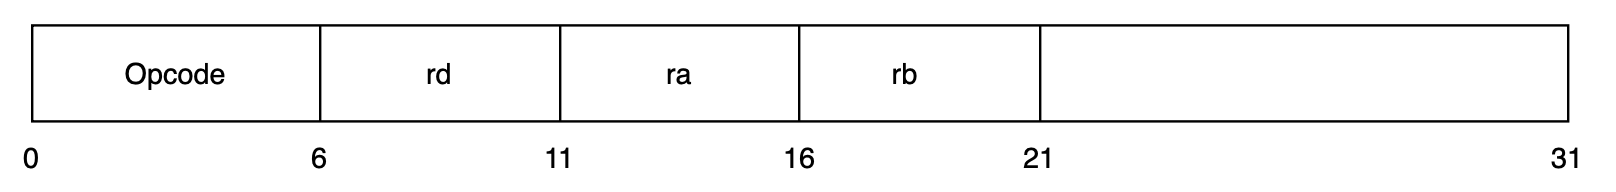
\includegraphics[scale=0.35]{images/Capitolo4/1_im.png}
    \caption{Type A istruction}
    \label{typeA}
    \end{figure}

    \item Type B:
    \begin{figure}[h!]
    \centering
    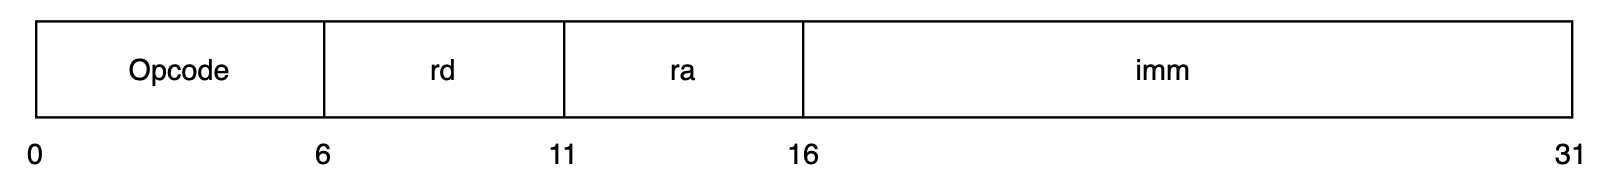
\includegraphics[scale=0.35]{images/Capitolo4/2_im.png}
    \caption{Type B istruction}
    \label{typeB}
    \end{figure}
\end{itemize}

\noindent Dove le componenti sono:

\begin{itemize}
    \item \texttt{Opcode}:\texttt{6 bit} per distinguere il tipo di istruzione.
    \item \texttt{rd}: \texttt{5 bit} per identificare il registro nel quale memorizzare il risultato dell'istruzione.
    \item \texttt{ra} e \texttt{rb}: ciascuno da \texttt{5 bit} come nel caso di \texttt{rd}, per identificare i due registri dove nel caso di una istruzione di tipo A, vengono utilizzati per eseguire l'operazione richiesta dall'istruzione. 
    \item \texttt{imm}: costituito \textbf{16 bit}, è presente sono nelle istruzioni di tipo B e viene utilizzato come fosse il registro \texttt{rb} nel caso delle istruzioni di tipo A. Questi bit identificano un valore immediato inserito direttamente nelle istruzioni assembler. Nel caso l'istruzione sia stata preceduta da una istruzione imm (\ref{imm}), viene esteso a 32 bit.
\end{itemize}

\vspace{0.3cm}

\noindent Di seguito l'implementazione della struttura che rappresenta le istruzioni:

\begin{lstlisting}[language=C]
struct Instruction 
{
    int8_t type : 1; /* 1 type A, 0 type B */
    int8_t opcode : 6;
    int8_t rd : 5;
    int8_t ra : 5;
    int8_t rb : 5;
    int32_t im : 32;
};
\end{lstlisting}
\label{structinstr}

\vspace{0.2cm}

\noindent L'interprete acquisisce le istruzioni da un file \texttt{.text}( sez \ref{compilazione}).  Queste istruzioni vengono caricate nell'interprete tramite la funzione (\ref{} ref apice) sottoforma di un array di puntatori a 4 interi di \texttt{8 bit}. Per elaborare le istruzioni l'interprete effettua il parsing di tali array per caricarli nella struttura \ref{structinstr} tramite la seguente funzione:

\begin{lstlisting}[language=C,label={parseinstr},caption={Parse Instruction}]
struct Instruction *parse_instruction(int8_t *instr, int8_t type, struct Instruction *res, int16_t *im)
{
	if (type) /* Type A */
	{
		res->type = type;
		res->rd = (instr[0] << 3) + ((instr[1] >> 5) & 0b00000111);
		res->ra = instr[1] & 0b00011111;
		res->rb = (instr[2] >> 3) & 0b00011111;
	}
	else /* Type B */
	{
		res->type = type;
		res->rd = ((instr[0] << 3) & 0b00011000) + ((instr[1] >> 5) & 0b00000111);
		res->ra = instr[1] & 0b00011111;
		int16_t n = instr[2];
		n = (n << 8) + (((int16_t)instr[3]) & 0b0000000011111111);

		if (*im) /* imm istruction before */
		{
			res->im = (*im << 16) + ((int32_t)n & 0b00000000000000001111111111111111);
			*im = 0;
		}
		else
			res->im = (int32_t)n;
	}
	return res;
}
\end{lstlisting}

Questa funzione accetta come parametri l'array della singola istruzione, il tipo della istruzione determinato a priori in base all'opcode, la struttura delle istruzioni da restuire dopo il parsing, e l'intero im (ovvero il registro in fig. \ref{structreg}). Nel caso l'istruzione sia preceduta da una istruzione imm (reference a imm),  come indicato nell'implementazione, il parametro viene usato per estendere l'immediato presente nella struttura a 32 bit. Questo viene fatto utilizzando i \texttt{16 bit} meno significativi dei bit dell'istruzione corrente, e i restanti bit più significativi dalla istruzione precedente imm. 
Si può notare come nel caso ci sia una istruzione di tipo A si rispetta la forma specificata in fig. \ref{typeA}, mentre nel caso di tipo B, si usa la specifica della fig. \ref{typeB}.

\vspace{0.3cm}

Prima di spiegare come alcune delle singole istruzioni sono state implementate, l'interprete al suo interno contiene delle funzioni di supporto per facilitare la scrittura di ogni singola implementazione di istruzione.

La prima funzione è la seguente: 
\begin{lstlisting}[language=C,label={updatepc},caption={Update PC}]
void update_PC(struct Registers *reg, int32_t n, bool delay)
{
    if (!delay)
        reg->pc = reg->pc + n / 4;
}
\end{lstlisting}

Questa funzione viene utilizzata per aggiornare lo stato del registro del Program Counter. Per facilità viene trattato come un numero intero. Tuttavia nella realtà e anche per il compilatore, per avanzare di un istruzione (dato che ogni istruzione occupa 4 byte) dividiamo il valore di 4. Questo permette di mantenere coerenza tra la rappresentazione del PC register nell'interprete e i comandi del compilatore.

Inoltre la CPU dispone istruzioni di salto che possono includere un flag di Delay Slot (\cite{libroarchitetture}). In caso questo flag di \texttt{Delay Slot} sia attivo, indipendentemente dal risultato del controllo dell'istruzione di salto, viene comunque eseguita l'istruzione successiva a quella in corso, a patto che questa non modifichi il Program Counter (come specificato nella documentazione \cite{sitoMicroblaze}. Tramite l'utilizzo di questo parametro nella funzione \texttt{update\_PC} manteniamo una corretta esecuzione del flusso del codice.

\clearpage

\noindent Un'altra funzione di supporto all'esecuzione dell'interprete è la seguente:
\begin{lstlisting}[language=C,label={convreg}]
int8_t conv_reg(int8_t n)
{
    return n & 0b00011111;
}
\end{lstlisting}

Questa funzione viene usata nel caso in cui il valore presente nella \texttt{struct Instructon} \ref{structinstr}, deve essere usato per operazioni bit a bit. 

Queste operazioni potrebbero non essere eseguite correttamente senza questa specifica conversione. Ciò è dovuto al fatto che qualsiasi operatore del linguaggio C, quando applicato come nel nostro caso a un intero \texttt{int8\_t}, il quale in realtà è un bit field da \texttt{5 bit} (come si nota in fig. \ref{structinstr}), utilizza tutti gli \texttt{8 bit} estendendo il nostro campo con dei bit non appropriati da \texttt{5} a \texttt{8}. Questo può portare a risultati inaspettati durante le operazioni.

Per risolvere questo problema, la funzione \texttt{conv\_reg} esegue una conversione, impostando correttamente i bit mancanti nel nostro campo. Questo assicura un utilizzo corretto degli operatori del linguaggio C senza gli errori derivanti da un estensione errata dei bit.

\vspace{0.3cm}

\noindent Come si può leggere nella documentazione \cite{sitoMicroblaze}, l'operazione fondamentale della CPU consiste nella somma di due registri. Questa operazione costituisce la base per gran parte delle istruzioni ed è l'unica che può causare overflow. Per gestire questo aspetto è stata implementata la seguente funzione:
\begin{lstlisting}[language=C]
int32_t add_Check_Overflow(int32_t a, int32_t b, bool *c)
{
    int64_t res = (int64_t)a + (int64_t)b; /* only last 32 bit*/
    if (res > INT32_MAX)
    {
        *c = true;
        res = INT32_MAX;
    }
    else if (res < INT32_MIN) /* underflow */
    {

        *c = true;
        res = INT32_MIN;
    }
    else
    {
        *c = false;
    }

    return (int32_t)res;
}
\end{lstlisting}
Questa funzione accetta due interi a \texttt{32 bit}, e il booleano \texttt{c}, il quale rappresenta il flag di carry dei registri, che viene settato in base a se si è o no verificato l'Overflow. 
Questi due interi vengono convertiti a \texttt{64 bit} per effettuare l'addizione, per poi controllare il risultato per vedere se sfora il massimo valore degli interi da \texttt{32 bit} oppure no.
Nel caso di questo interprete viene anche gestito l'Underflow.

La base dell'interprete stesso è una funzione chiamata \texttt{run\_instruction}. All'interno di questa funzione è presente uno switch, il quale in base all'opcode situato nei primi \texttt{6 bit} dell'istruzione, seleziona il caso appropriato per eseguire l'operazione corrispondente. 

\vspace{0.3cm}
\noindent L'implementazione della funzione è la seguente:

\begin{lstlisting}[language=C,caption={Run Instruction},label={runinstruction}]
void run_instruction(int8_t *instruction, 
                    struct Memory *data, 
                    struct Registers *reg, 
                    int8_t **instructions, 
                    bool delay)
{
	struct Instruction *instr = malloc(sizeof(struct Instruction));
	bool carry = 0; //carry
    op_code = (instruction[0] >> 2) & 0b00111111;
	instr->opcode = op_code;
	int32_t delayed_instruction, addr;
	int8_t branch_type, is_delayed, is_absolute, is_link;

	switch (op_code) {
		...
    }
}
\end{lstlisting}
Questa funzione accetta come parametri l’array della singola istruzione, lo stato corrente della memoria e dei registri, l'array contenente tutte le istruzioni (che viene utilizzato nelle istruzioni con delay per effettuare una ricorsione, come nella fig. \ref{branch}), e un booleano Delay Slot. Quando viene eseguita un istruzione con delay, il parametro impedisce l'aggiornamento del Program Counter nella funzione \texttt{update\_pc}. (come visto nella fig. \ref{updatepc})

\vspace{0.3cm}

All'inizio della funzione viene creata un istanza che rappresenta le istruzioni dopo il parsing della funzione \texttt{parse\_instruction} (fig. \ref{parseinstr}).
All'interno di questa struttura, il parametro \texttt{op\_code}, viene inizializzato per motivi di facilità, poiché è utilizzato immediatamente. Successivamente vengono create le istanze delle variabili utilizzate all'interno dei vari case dello switch, le quali verranno spiegate successivamente.

\vspace{0.3cm}

Segue una spiegazione dei vari casi dello switch. Per evitare di ripetizioni, verranno illustrate solo le parti principali, poiché la maggior parte degli altri casi presentano solo delle variazioni minori.

\vspace{0.3cm}

La prima funzione dello switch è la \texttt{ADD} ed è implementata come segue:
\begin{lstlisting}[language=C]
  case 0x0 : 
  { /* ADD 000000 */
    instr = parse_instruction(instruction, TYPE_A, instr, &reg->im);
    reg->r[instr->rd] = add_Check_Overflow(reg->r[instr->ra], reg->r[instr->rb], &carry);
    update_PC(reg, 4, delay);
    break;
  }
\end{lstlisting}
Questo caso rappresenta in gran parte la struttura di tutte le istruzioni. Notare che i casi sono abbinati agli opcode scritti in esadecimale per una questione di leggibilità. L'esecuzione inizia chiamando la funzione per il parsing dell'istruzione, con i parametri appropriati. Secondo la documentazione, l'istruzione \texttt{ADD} è una di tipo A, per cui si chiama con la variabile \texttt{TYPE\_A} definita all'inizio dell'interprete. Successivamente per eseguire l'operazione effettiva, viene utilizzata la funzione di supporto \texttt{ add\_Check\_Overflow}, che assicura la gestione dell'overflow e dell'eventuale bit di carry.

È importante notare che, nel caso dell'istruzione \texttt{ADD}, la CPU Microblaze non tiene conto del bit di carry né per fare la somma e né per salvarlo in caso di carry effettivo.
Possiamo osservare che il funzionamento effettivo consiste nell'eseguire la somma del contenuto del registro \texttt{ra} con il registro \texttt{rb}, e successivamente di memorizzare il risultato nel registro \texttt{rd}.
Si osserva come al termine dell'esecuzione, venga effettuato l'aggiornamento del Program Counter per puntare alla istruzione successiva.

\vspace{0.3cm}

\noindent Per gestire questa situazione, è utile osservare l'implementazione che segue dell'istruzione \texttt{ADDCK}:
\begin{lstlisting}[language=C]
  case 0x6:
  { /* ADDCK 000110 */
   instr = parse_instruction(instruction, TYPE_A, instr, &reg->im);
   reg->r[instr->rd] = add_Check_Overflow(reg->r[instr->ra], reg->r[instr->rb] + reg->c, &carry);
   reg->c = carry;
   update_PC(reg, 4, delay);
   break;
  }
\end{lstlisting}
Possiamo notare come la struttura del rimane invariata rispetto alla istruzione. Come anche il nome dell'istruzione implica, questa variante dell'istruzione \texttt{ADD}, tramite il flag \texttt{C} (nel nome della istruzione) tiene conto del bit di carry precedentemente salvato, per effettuare l'operazione di somma, e con il flag \texttt{K} ovvero "keep", implica il salvataggio dell'eventuale bit di carry nello stato dei registri generato dall'operazione.

\noindent Di seguito l'implementazione dell'istruzione \texttt{RSUB}: 
\begin{lstlisting}[language=C]
 case 0x1:
 { /* RSUB 000001 */
    instr = parse_instruction(instruction, TYPE_A, instr, &reg->im);
    reg->r[instr->rd] = add_Check_Overflow(reg->r[instr->rb], add_Check_Overflow(~reg->r[instr->ra], 1, &carry), &carry);
    update_PC(reg, 4, delay);
    break;
 }
\end{lstlisting}
Si noti una differenza fondamentale rispetto alla istruzione \texttt{ADD}: qui viene eseguita un somma tra il contenuto del registro \texttt{rb} e il not del contenuto del registro \texttt{ra} sommato a 1. Ovvero la sottrazione è implementata come somma del complemento a due del secondo operando. Questo approccio per effettuare la sottrazione è stato adottato per rispettare il funzionamento specificato nella documentazione \cite{sitoMicroblaze}.
Nonostante questo cambiamento il paradigma di esecuzione rimane invariato. Da notare che anche questa istruzione presenta le varianti \texttt{RSUBC}, \texttt{RSUBK} e \texttt{RSUBCK}.

\vspace{0.3cm}

\noindent Sia l'istruzione \texttt{ADD} che l'istruzione \texttt{RSUB} presentano le rispettive varianti \texttt{ADDI} e \texttt{RSUBI} per gestire il caso dei valori immediati, entrambe con le varianti con i vari flag per il bit di carry presenti. Di seguito, l'implementazione dell'istruzione \texttt{ADDI}:

\begin{lstlisting}[language=C]
 case 0x8:
 { /* ADDI 001000 */
    instr = parse_instruction(instruction, TYPE_B, instr, &reg->im);
    reg->r[instr->rd] = add_Check_Overflow(instr->im, reg->r[instr->ra], &carry);
    update_PC(reg, 4, delay);
    break;
 }
\end{lstlisting}
Possiamo notare pur essendo la stessa istruzione, al posto del registro \texttt{rb} è presente il valore immediato \texttt{instr->im}, il quale viene utilizzato come operando per l'operazione di somma. 
Per il resto il flusso dell'esecuzione rimane invariata.

\vspace{0.3cm}

L'interprete presenta la possibilità di eseguire operazioni bit a bit tramite le istruzioni offerte dall'architettura RISC, tra cui \texttt{AND}, \texttt{OR}, \texttt{SRA}, \texttt{XOR}, e cosi via.
Anche queste presentano lo stesso paradigma di esecuzione delle istruzione precedenti, come è possibile osservare dall'implementazione seguente: 

\begin{lstlisting}[language=C]
case 0x22:
{ /* XOR 100010 */
    instr = parse_instruction(instruction, TYPE_A, instr, &reg->im);
    reg->r[instr->rd] = reg->r[instr->ra] ^ reg->r[instr->rb];
    update_PC(reg, 4, delay);
    break;
}
\end{lstlisting}

Nel caso in cui nel linguaggio assembly venga inserito un immediato che superi i 16  bit di grandezza, ovvero la dimensione riservata ai valori immediati nelle istruzioni di tipo B (fig. \ref{typeB}), il compilatore aggiunge, dopo il processo di compilazione, l'istruzione \texttt{imm}. Questa istruzione estende l'immediato dell'istruzione che la posticipa a 32 bit, nel modo specificato nella spiegazione della funzione \texttt{parse\_instruction} (fig. \ref{parseinstr}). L'implementazione di tale istruzione è la seguente:

\begin{lstlisting}[language=C]
 case 0x2C:
 { /* IMM 101100 */
    instr = parse_instruction(instruction, TYPE_B, instr, &reg->im);
    reg->im = instr->im;
    update_PC(reg, 4, delay);
    break;
 }
\end{lstlisting}
\label{imm}

\vspace{0.3cm} 

Le uniche istruzioni utilizzate da questo interprete per gestire la memoria dati sono \texttt{LW} e \texttt{SW}, entrambe con le varianti \texttt{LWI} e \texttt{SWI} per gestire il caso degli immediati.

\noindent Segue la loro implementazione:
\begin{lstlisting}[language=C]
 case 0x32:
 { /* LW 110010 */
    instr = parse_instruction(instruction, TYPE_A, instr, &reg->im);
    addr = (uint32_t)(reg->r[instr->ra] + reg->r[instr->rb]);
    reg->r[instr->rd] = data->data[addr];
    update_PC(reg, 4, delay);
    break;
 }
 case 0x36:
 { /* SW 110110 */
    instr = parse_instruction(instruction, TYPE_A, instr, &reg->im);
    addr = (uint32_t)(reg->r[instr->ra] + reg->r[instr->rb]);
    data->data[addr] = reg->r[instr->rd];
    update_PC(reg, 4, delay);
    break;
 }
\end{lstlisting}
Osserviamo che entrambe queste istruzioni effettuano una somma tra il registro \texttt{ra} e il registro \texttt{rb} per ottenere l'indirizzo di memoria. Nel caso dell'istruzione \texttt{LW} salviamo nel registro \texttt{rd} il contenuto della memoria all'indirizzo precedentemente calcolato dentro la variabile \texttt{addr}, mentre nel caso di \texttt{SW} facciamo esattamente il contrario, ossia salviamo in memoria il contenuto del registro \texttt{rd} all'indirizzo precedentemente calcolato.
Nella versione \texttt{SWI} e \texttt{LWI} l'unica differenza (oltre al tipo di istruzione, che diventa di tipo B), è la seguente riga:
\begin{lstlisting}[language=C]
 ...
 addr = (uint32_t)(reg->r[instr->ra] + instr->im);
 ...
\end{lstlisting}
Si nota come al posto del registro \texttt{rb} venga usato semplicemente il valore immediato.

Notare come l'indirizzo \texttt{addr} viene sempre usato come un \texttt{unsigned int} a \texttt{32 bit}. Questo perché la memoria dati è un array, e l'indicizzazione inizia da \texttt{0} e cosi via in maniera sequenziale, di conseguenza l'utilizzo di questi cast assicura la corretta esecuzione del codice.

\vspace{0.3cm}

Le istruzioni di salto gestite da questo interprete si distinguono, come le altre istruzioni, in due categorie: quelle che gestiscono gli immediati, contrassegnate dal flag \texttt{I} nel nome, e quelle senza immediati, ovvero con l'utilizzo di registri normali. 

Di seguito la loro implementazione:
\begin{lstlisting}[language=C,label={branch},caption={Istruzioni Branch}]
 case 0x27:
 { /* BEQ BGE BGT BLE BLT BNE 100111 */
    instr = parse_instruction(instruction, TYPE_A, instr, &reg->im);
    delayed_instruction = reg->pc + 1;  /* prossima istruzione da eseguire in caso di delay*/
    branch_type = conv_reg(instr->rd) & 0b00001111;
    is_delayed = conv_reg(instr->rd) & 0b00010000;

  if ((branch_type == 0x0 && reg->r[instr->ra] == 0x0) || /* BEQ D0000 */
    (branch_type == 0x5 && reg->r[instr->ra] >= 0x0) || /* BGE D0101 */
    (branch_type == 0x4 && reg->r[instr->ra] >  0x0) ||	/* BGT D0100 */
    (branch_type == 0x3 && reg->r[instr->ra] <= 0x0) || /* BLE D0011 */
    (branch_type == 0x2 && reg->r[instr->ra] <  0x0) ||	/* BLT D0010 */
    (branch_type == 0x1 && reg->r[instr->ra] != 0x0))		/* BNE D0001 */
        update_PC(reg, reg->r[instr->rb], delay);
  else
        update_PC(reg, 4, delay);

  if (is_delayed == 0x10) /* delayed slot */
    run_instruction(instructions[delayed_instruction], data, reg, instructions, true);
 break;
 }
\end{lstlisting}
Si nota come l'opcode sia lo stesso per tutte le istruzioni di branch (come specificato nella documentazione \cite{sitoMicroblaze}). Il tipo specifico di ciascuna lo si ricava dai 4 bit meno significativi del registro \texttt{rd} (come specificato nella documentazione \cite{sitoMicroblaze}).
Possiamo vedere come a seconda di quale sia il tipo di branch da eseguire, specificato nella variabile \texttt{branch\_type}, andiamo ad eseguire il controllo appropriato del contenuto del registro \texttt{ra}, per poi aggiornare il valore del pc register con il valore contenuto nel registro \texttt{rb}.
Successivamente, nel caso in cui l'istruzione abbia il flag \texttt{D} nel nome, che imposta a \texttt{1} il quinto bit del registro \texttt{rd}, si procede con l'esecuzione dell'istruzione successiva a quella del branch, senza tener conto se il controllo è andato a buon fine. Questo viene fatto impostando a true il parametro del delay slot, evitando cosi di aggiornare il pc register mentre eseguiamo questa istruzione, per poi riprendere il normale flusso del programma.

\vspace{0.5cm}

\noindent Fino a questo punto abbiamo esaminato le varie parti dell'interprete. Tuttavia nel contesto di un programma tutto ciò va utilizzato seguendo il flusso di una normale CPU. Per questo per sfruttare la funzione \texttt{run\_instruction}, si utilizza un ciclo che prosegue fino a quando program counter non raggiunge l'ultima istruzione della lista.
Di seguito è riporta l'implementazione di questo ciclo:
\begin{lstlisting}[language=C,caption={Ciclo Interprete},label={ciclointerprete}]
while (reg->pc < instructions_size) { 
    run_instruction(instructions[reg->pc], 
                        data, 
                        reg, 
                        instructions, 
                        false);
}
\end{lstlisting}

Inoltre per far funzionare l'interprete, è necessario disporre del bytecode delle istruzioni assembler generato dal compilatore, (come mostrato nella figura \ref{funzionamentoOpenCL}.
Per fare ciò, il metodo usato è il seguente. 
Partendo da un file \texttt{.s}, di seguito viene riportato un esempio di codice assembler:

\begin{lstlisting}
	.text
	.align	2
	.globl	main
	.ent	main
	.type	main, @function  

main:
	addi	r2,r0,55 
	addi	r3,r0,100
	cmp     r4,r2,r3 
	addi	r5,r0,2147483640
	
	.end	main
\end{lstlisting}
Successivamente utilizzando del compilatore fornito da Xilinx, \texttt{mb-gcc}, il codice viene compilato in un file \texttt{.o}.

\vspace{0.3cm}

\noindent Possiamo vedere il codice assembly disassemblato tramite il seguente comando: 

\begin{lstlisting}
mb-objdump -d assembler.o
\end{lstlisting}
Notare si utilizza il tool \texttt{objdump} offerto da Xilin. Il risultato del comando è il seguente:

\begin{lstlisting}
00000308 <main>:
 308:	20400037 	addi	r2, r0, 55
 30c:	20600064 	addi	r3, r0, 100
 310:	14821801 	cmp	r4, r2, r3
 314:	b0007fff 	imm	32767
 318:	20a0fff8 	addi	r5, r0, -8
\end{lstlisting}
Notare come il compilatore aggiunge l'istruzione \texttt{imm} per estendere l'immediato della istruzione \texttt{addi}. 
Possiamo notare come questa sezione del file \texttt{.o} contiene il bytecode delle istruzioni tradotte dall'assembler a codice macchina.
A questo punto è possibile estrarre solamente la sezione \texttt{.text} attraverso l'utilizzo del tool \texttt{objcopy}. 

\vspace{0.3cm}

\noindent Questo processo avviene attraverso i comandi seguenti:
\begin{lstlisting}[language=Bash]
	mbgcc -o assemler.o -c assembler.s 
	objcopy -j .text -O binary -I elf32-little assembler.o assembler.text  
\end{lstlisting}
\label{estrazioneBytecode}

\section{Interprete Versione Kernel}
\label{Interprete Kernel}
In questa sezione, saranno dettagliate tutte le modifiche apportate all'interprete per renderlo compilabile ed eseguibile sulla scheda FPGA. 

\vspace{0.3cm}
\noindent Il codice completo relativo alla sezione seguente è presente nell'appendice (ref a vadd.cpp)
\vspace{0.3cm}

\noindent Finora, il codice dell'interprete sfrutta ampiamente i paradigmi offerti da un linguaggio di alto livello come il C.
Tuttavia va sottolineato che non è possibile utilizzare molti di questi paradigmi per sviluppare un kernel compilabile ed eseguibile su una scheda FPGA. Questo perché la generazione tramite High-Level Synthesis (HLS) messa a disposizione da Vitis, impone restrizioni specifiche che devono essere rispettate per completare il processo di compilazione del kernel e garantire il suo corretto funzionamento.

\vspace{0.3cm}

Durante la conversione dell'interprete al paradigma di funzionamento di un kernel sono stati riscontrati due problemi. In primo luogo, non è permesso l'uso di doppi puntatori, e in secondo luogo, non è possibile utilizzare chiamate ricorsive. Questi vincoli hanno creato due problemi, il primo riguarda la dichiarazione delle istruzioni, le quali come già precedentemente descritto precedentemente (\ref{structinstr}), sono definite come un puntatore di puntatori a interi da \texttt{8 bit}. Questo è stato risolto dichiarando a priori la dimensione massima del vettore delle istruzioni (ovvero il programma assembler) e quindi utilizzando la definizione di una matrice invece che un doppio puntatore. Come si può vedere nella seguente maniera: 
\begin{lstlisting}[language=C]
#define MAX_INSTR 32
    
int8_t instr[MAX_INSTR][4];
\end{lstlisting}
Come si può notare, possiamo gestire fino 32 istruzioni, una quantità che comunque può essere cambiata, e che si è dimostrata più che sufficiente per gli scopi di test di questo interprete. 

\vspace{0.3cm}

Il problema delle chiamate ricorsive è stato risolto eliminando le istruzioni che facevano uso del delay slot. Questa decisione è stata presa perché non era un obbiettivo primario di questa tesi, e inoltre anche per mantenere l'implementazione relativamente semplice e focalizzata sugli aspetti essenziali del funzionamento di una FPGA.
Una possibile soluzione consiste nel aggiungere un parametro nella funzione \texttt{run\_instruction} (fig. \ref{runinstruction}). Questo parametro viene verificato ad ogni iterazione del ciclo dell'interprete (fig. \ref{ciclointerprete}), e se attivo, consente l'esecuzione dell'istruzione presente nel Delay Slot, per poi tornare al normale flusso di esecuzione.

\vspace{0.3cm}

\noindent Successivamente alla risoluzione di questi problemi, la procedura per sviluppare un kernel richiede la scrittura di una funzione che viene chiamata  all'avvio dell'esecuzione sulla FPGA. 
Procediamo con il far vedere la segnatura della funzione:
\begin{lstlisting}[language=C]
void interprete(struct Memory *mem, 
                struct Registers *reg, 
                int32_t *out, 
                ap_uint<32> my_size) 
{
   ...
}
\end{lstlisting}
Questa funzione prende come parametri la struttura della memoria, la struttura dei registri, un intero da \texttt{32 bit} chiamato \texttt{out} per restituire il risultato  e \texttt{my\_size} che rappresenta la grandezza delle istruzioni. Questa scelta di utilizzare un singolo valore per verificare il corretto funzionamento è stata fatta poiché ai fini dei test iniziali è stato sufficiente restituire il risultato dell'esecuzione salvato in un singolo registro.
Notare come in generale il risultato dell'esecuzione del codice sarà rappresentato nella memoria dati, che alla fine della computazione viene ricopiata nella memoria host, come vedremo nella sez. \ref{interpretegpu}
Notare che per ridurre la quantità di parametri, le istruzioni sono state caricate insieme alla memoria \texttt{mem}.
Notare che questi parametri sono dichiarati e inizializzati dal lato host, questo aspetto verrà spiegato nella sezione \ref{host}.

\vspace{0.3cm}

\noindent Appena all'inizio della funzione \texttt{interprete}, sono presenti le seguenti specifiche:

\begin{lstlisting}[language=C]
...
#pragma HLS INTERFACE m_axi port = mem bundle = gmem
#pragma HLS INTERFACE m_axi port = reg bundle = gmem
#pragma HLS INTERFACE m_axi port = out bundle = gmem
#pragma HLS INTERFACE ap_ctrl_hs port = return
...
\end{lstlisting}

Queste righe di codice sono delle direttive chiamate "HLS pragmas". Queste rappresentano delle specifiche HLS per il compilatore \texttt{v++}, utilizzato nella fase di sintesi hardware (\ref{compilazione}). Queste direttive specificano come avviene la creazione delle porte RTL, a partire dagli argomenti della funzione durante la sintesi dell'interfaccia. Queste porte rappresentano il punto di connessione tra l'hardware presente nel chip della FPGA e le strutture esterne, come in questo caso la memoria globale DDR presente nella scheda che ospita il chip dell'acceleratore.
Facendo cosi il tool HLS determina automaticamente i protocolli I/O usati per gestire lo scambio di informazioni tra la parte acceleratore e i gli altri componenti del sistema.

L'utilizzo di queste direttive consente di determinare automaticamente i protocolli I/O utilizzati per la gestione dello scambio di informazioni tra la parte acceleratore e gli altri componenti. In questo caso specifico (come specificato nella documentazione \cite{sitoDocumentazionePragma}), le prime tre direttive \texttt{m\_axi} definiscono le interfacce di tipo master AXI4 (Advanced Extensible Interface), per le strutture \texttt{mem}, \texttt{reg} e \texttt{out}. Tutte queste porte sono tutti blocchi AXI, hanno tutti un bit che dice quando la computazione è terminata, la quarta direttiva \texttt{ap\_ctrl\_hs)}, specifica di impostare a 1 il bit del blocco quando si esegue il comando \texttt{return}.

\vspace{0.3cm}

Successivamente alle direttive \texttt{\#pragma} nella funzione è presente il seguente codice:
\begin{lstlisting}[language=C,caption={Funzione Interprete},label={funzioneinterprete}]
...
  struct Registers reg_copy;
  struct Memory mem_copy;
  
  // Copia dei registri dalla memoria globale alla memoria locale
  for (int i = 0; i < 32; i++)
    reg_copy.r[i] = reg->r[i];
  reg_copy.c = reg->c;
  reg_copy.pc = reg->pc;
  reg_copy.im = reg->im;

  // Copia della memoria dalla memoria globale alla memoria locale
  for (int i = 0; i < 1024; i++)
    mem_copy.data[i] = mem->data[i];

  for (int i = 0; i < MAX_INSTR; i++)
    for (int j = 0; j < 4; j++)
        mem_copy.instr[i][j] = mem->instr[i][j];
        
  // Creazione dei puntatori per accedere alle copie locali      
  struct Registers *reg_copy_pointer = &reg_copy;
  struct Memory *mem_copy_pointer = &mem_copy;

  // Ciclo interprete
  while (reg_copy_pointer->pc < my_size)
    run_instruction(mem_copy_pointer->instr[reg_copy_pointer->pc], 
        mem_copy_pointer, 
        reg_copy_pointer, 
        mem_copy_pointer->instr, 
        false);
        
  // Restituzione del risultato al lato host
  *out = reg_copy_pointer->r[1];
}
\end{lstlisting}
Come è possibile notare dall'implementazione, viene eseguita una copia locale dei parametri provenienti dal lato host e caricati sulla DDR attraverso strutture allocate staticamente, cosi facendo queste strutture dati risulteranno allocate nei blocchi RAM interni alla FPGA stessa (come sarà dimostrato nella sez. \ref{utilizzofpga}). Questo per evitare errori generati a tempo di esecuzione del kernel sulla FPGA, Successivamente le copie locali dei parametri, ovvero \texttt{reg\_copy} e \texttt{mem\_copy}, vengono usate tramite puntatori al fine di mantenere la leggibilità del codice e la coerenza. Successivamente è presente un ciclo, che come già precedentemente spiegato \ref{Interprete Softcore} permette  di proseguire fino a quando il registro program counter non raggiunge l’ultima istruzione della lista.

Alla fine del ciclo viene eseguita una copia del registro \texttt{r1} sul parametro esterno \texttt{out} per restituire il valore del risultato della computazione.

Come già specificato precedentemente, il resto del codice rispetto alla versione spiegata nella sezione \ref{Interprete Softcore}, rimane invariato.

\section{Interfaccia Host}
\label{host}
In questa sezione saranno dettagliate le componenti e il loro funzionamento dell'interfaccia usata sulla macchina host per gestire il trasferimento dei dati e la computazione della scheda FPGA.

\vspace{0.3cm}

\noindent Il codice completo relativo alla sezione seguente è presente nell'appendice (\ref{codicehost1cu})

\vspace{0.3cm}

\noindent In questa sezione del codice, avvengono tutte le chiamate OpenCl per interfacciarsi con l'acceleratore FPGA. 
Il funzionamento generale è riassunto nel seguente workflow: 
\begin{enumerate}
    \item Acquisire il file \texttt{.xclbin}, risultante dalla sintesi hardware del kernel dell'interprete (\ref{compilazione}) e il file \texttt{.text} derivante dall'estrazione del bytecode da un programma scritto in assembler (\ref{estrazioneBytecode}).
    \item Preparare l'ambiente di esecuzione e caricare i dati nella memoria DDR della FPGA.
    \item Procedere con l'esecuzione della computazione all'interno dell'acceleratore FPGA.
    \item In fine estrarre i risultati dalla memoria DDR e restituirli.
\end{enumerate}

\vspace{0.3cm}

Per capirne il funzionamento iniziamo analizzando la porzione iniziale di codice dove vengono istanziate tutte le variabili necessarie per questa procedura:

\begin{lstlisting}[language=C++]
int main(int argc, char **argv)
{
	// Verfica numero argomenti
	if (argc != 2)
	{
		std::cout << "Usage: " << argv[0] << " <XCLBIN File>" << std::endl;
		return EXIT_FAILURE;
	}

	// Dichiarazione Variabili Opencl
	cl_int err;
	cl::CommandQueue q;
	cl::Context context;
	cl::Kernel krnl;
 
	bool valid_device = false;

	// Allocazione spazio risultato
	int32_t *result = (int32_t*)malloc(sizeof(int32_t));
	*result = 0;

	// Lettura dispositvo 
	auto devices = xcl::get_xil_devices();

	// Creazione binario OpenCL 
	std::string binaryFile = argv[1];
	auto fileBuf = xcl::read_binary_file(binaryFile);
	cl::Program::Binaries bins{{fileBuf.data(), fileBuf.size()}};
...
\end{lstlisting}
Si nota che il file \texttt{.xclbin} viene passato come argomento alla funzione \texttt{main} all'avvio dell'eseguibile.
Successivamente, vengono dichiarate le variabili OpenCL necessarie, tra cui:
\begin{itemize}
    \item \texttt{cl\_int err;}: utilizzata per la  verifica dei possibili errori derivanti dalle chiamate di funzione OpenCL.
    \item \texttt{cl::CommandQueue q}: rappresenta una coda dei comandi. In OpenCL una variabile di questo tipo viene utilizzata per inoltrare dei comandi all'acceleratore (FPGA in questo caso) per l'esecuzione di operazioni.
    \item \texttt{cl::Context context}: rappresenta il contesto OpenCL, ovvero un oggetto dove è possibile creare e gestire la memoria dedicata per l'acceleratore, caricare i kernel da eseguire, e  altro ancora.
    \item \texttt{cl::Kernel krnl}: rappresenta un kernel OpenCL, ovvero il programma che sarà eseguito dall'acceleratore nel formato binario specifico del dispositivo.
\end{itemize}

In seguito, osserviamo alcune chiamate di funzione dalla libreria \texttt{xcl}, il quale è il runtime driver fornito da Xilinx. 
In generale il loro funzionamento è il seguente:
\begin{itemize} 
    \item \texttt{xcl::get\_xil\_devices()}: restituisce una lista di dispositivi compatibili con la piattaforma Xilinx.
    \item \texttt{xcl::read\_binary\_file(binaryFile)} restituisce un buffer a partire dal contenuto del file \texttt{.xclbin}.
\end{itemize}

Successivamente viene creato un oggetto "\texttt{cl::Program::Binaries bins}", il quale rappresenta il contenuto binario di un programma OpenCL.

Di seguito il codice per effettuare la programmazione dei dispositivi di accelerazione:
\begin{lstlisting}[language=C++,caption={ricerca dispositi},label={lst:ricerca}]
...
 for (unsigned int i = 0; i < devices.size(); i++)
 {
    auto device = devices[i];   
    
    // Creazione della coda di comando e del contesto per i device presenti
    OCL_CHECK(err, context = cl::Context(device, nullptr, nullptr, nullptr, &err));
    OCL_CHECK(err, q = cl::CommandQueue(context, device, CL_QUEUE_PROFILING_ENABLE, &err)); 
    std::cout << "Trying to program device[" << i << "]: " << device.getInfo<CL_DEVICE_NAME>() << std::endl;
    cl::Program program(context, {device}, bins, nullptr, &err);    
    
    if (err != CL_SUCCESS)
    {
        std::cout << "Failed to program device[" << i << "] with xclbin file!\n";
    }
    else
    {
        std::cout << "Device[" << i << "]: program successful!\n"; 
        
        //Creazione Kernel
        OCL_CHECK(err, krnl = cl::Kernel(program, "interprete", &err)); 
        valid_device = true;
        break; // Device valido trovato
    }
 }
...
\end{lstlisting}
Possiamo osservare come per ogni dispositivo (nel nostro caso è sempre stato solo uno, ovvero l'FPGA), vengono creati il contesto e la coda di comando utilizzando le funzioni di supporto di OpenCL. Inoltre viene creato l'oggetto \texttt{program}, , il quale rappresenta il programma che sarà eseguito nell'FPGA. Una volta creato il programma, viene utilizzato per creare il kernel, nel quale durante la creazione, specifichiamo il nome della funzione che verrà chiamata all'avvio dell'esecuzione.
Notare come eventuali errori vengo gestiti e registrati nella variabile \texttt{err}.

Successivamente vengono caricate le istruzioni dal file \texttt{.text}, vengono inizializzati memoria e registri dell'interprete, e le istruzioni vengono copiate all'interno della memoria dati. Di seguito è riportato il codice corrispondente: 

\begin{lstlisting}[language=C++]
...
 int32_t instr_size = 0;
 int8_t **instr_vector = get_instructions_from_file(file, &instr_size);
 auto mysize = instr_size;

 struct Memory *data = (struct Memory *)malloc(sizeof(struct Memory));
 struct Registers *reg = (struct Registers *)malloc(sizeof(struct Registers));

 // Inizializzazione Registri
 reg = inizialize_registers(reg);

 // Inizializzazione Memoria
 for (int i = 0; i < 1024; i++)
    data->data[i] = 0;

 // Copia istruzioni
 for (int i = 0; i < mysize; i++)
 {
    data->instr[i][0] = instr_vector[i][0];
    data->instr[i][1] = instr_vector[i][1];
    data->instr[i][2] = instr_vector[i][2];
    data->instr[i][3] = instr_vector[i][3];
 }
 ...
\end{lstlisting}

\vspace{0.3cm}

\noindent Successivamente si trova l'ultima sezione del codice dell'interfaccia host, dove continua la gestione della memoria e inizia la computazione dell'acceleratore, di seguito l'implementazione di questa: 
\begin{lstlisting}[language=C++]
...
 // Allocazione Buffer nella memoria globale della FPGA
 OCL_CHECK(err, cl::Buffer buffer_out(context, CL_MEM_USE_HOST_PTR | CL_MEM_WRITE_ONLY, sizeof(int32_t), result, &err));
 OCL_CHECK(err, cl::Buffer buffer_data(context, CL_MEM_USE_HOST_PTR | CL_MEM_READ_ONLY, sizeof(struct Memory), data, &err));
 OCL_CHECK(err, cl::Buffer buffer_reg(context, CL_MEM_USE_HOST_PTR | CL_MEM_READ_ONLY, sizeof(struct Registers), reg, &err));

 // Configurazione degli argomenti del kernel
 OCL_CHECK(err, err = krnl.setArg(0, buffer_data));
 OCL_CHECK(err, err = krnl.setArg(1, buffer_reg));
 OCL_CHECK(err, err = krnl.setArg(2, buffer_out));
 OCL_CHECK(err, err = krnl.setArg(3, mysize));

 // Migrazione dei dati dalla memoria host alla memoria globale della FPGA
 OCL_CHECK(err, err = q.enqueueMigrateMemObjects({buffer_data, buffer_reg}, 0 /*from host*/));

 // Inizio esecuzione kernel
 OCL_CHECK(err, err = q.enqueueTask(krnl));

 // Migrazione risultati dall'acceleratore alla memoria host 
 OCL_CHECK(err, err = q.enqueueMigrateMemObjects({buffer_out}, CL_MIGRATE_MEM_OBJECT_HOST));

 // Attesa che il kernel completi l'esecuzione
 OCL_CHECK(err, err = q.finish());

 std::cout << "\n\n FPGA RESULT " << *result << "\n\n";

 return EXIT_SUCCESS;
}
\end{lstlisting}
Si nota come inizialmente, si creano oggetti di tipo \texttt{cl::Buffer}, i quali rappresenta buffer di memoria sulla FPGA. Successivamente, gli argomenti della funzione iniziale presente nel kernel vengono configurati correttamente, in modo da fornire gli input nell'ordine appropriato. Viene quindi utilizzata la funzione \texttt{enqueueMigrateMemObjects} per aggiungere alla coda di comandi il comando che migra i dati dai buffer \texttt{buffer\_data} e \texttt{buffer\_reg} dalla memoria host alla memoria della FPGA (notare come l'argomento 0 specifica la direzione della migrazione). Successivamente, viene aggiunto alla coda di comando per avviare l'esecuzione del kernel.
L'istruzione \texttt{q.finish()} è utilizzata per attendere che tutte le operazioni all'interno della coda finiscano prima di proseguire con il resto del codice.
Una volta eseguite le operazione il risultato viene stampato e il programma termina.

\clearpage

\section{Compilazione}
\label{compilazione}
Vitis mette a disposizione 3 modi di compilare il progetto tramite il compilatore da loro offerto \texttt{v++}:

\begin{itemize}
    \item \textbf{Software Emulation}: in questa modalità, il kernel è compilato per essere eseguito sulla CPU della macchina host. Questo processo permette di rifinire facilmente il codice attraverso step iterativi di cicli build-and-run.
    \item \textbf{Hardware Emulation}: in questa modalità, il kernel viene compilato nel modello hardware (RTL), il quale viene eseguito in emulatore dedicato. Sebbene il processo di compilazione richieda più tempo, fornisce dettagli più approfonditi sull'esecuzione del kernel, e delle performance.
    \item \textbf{Hardware}: in questo processo il kernel viene compilato nell'hardware model (RTL) e viene implementato direttamente nella FPGA.
\end{itemize}
    
La prima fase del processo di compilazione, come indicato nella documentazione \cite{sitoDocumentazioneVitis}, consiste nel configurare l'ambiente per eseguire Vitis. Si utilizzano i seguenti comandi: 
\begin{lstlisting}[language=Bash]
source /tools/Xilinx/Vitis/2023.1/settings64.sh
source /opt/xilinx/xrt/setup.sh
\end{lstlisting}

Successivamente è necessario configurare correttamente la seguente variabile di ambiente: 
\begin{lstlisting}[language=Bash]
export PLATFORM_REPO_PATHS=/opt/xilinx/platforms/xilinx_u50_gen3x16_xdma_5_202210_1/
\end{lstlisting}
Questa variabile di ambiente indica il percorso per le piattaforme istallate sulla macchina corrente. Possiamo notare come la nostra piattaforma sia la scheda \texttt{u50}.

Successivamente il processo continua tramite i seguenti comandi:
\begin{lstlisting}[language=Bash]
export XCL_EMULATION_MODE=sw_emu
g++ -g -std=c++17 -Wall -O0 src/host.cpp src/xcl2.cpp -o ./app.exe -I$XILINX_XRT/include/ -L$XILINX_XRT/lib -lxrt_coreutil -pthread -lOpenCL
emconfigutil --platform xilinx_u50_gen3x16_xdma_5_202210_1
v++ -c -t sw_emu --platform xilinx_u50_gen3x16_xdma_5_202210_1 -k vadd -I/src src/vadd.cpp -o ./vadd.xo
v++ -l -t sw_emu --platform xilinx_u50_gen3x16_xdma_5_202210_1 ./vadd.xo -o ./vadd.xclbin
\end{lstlisting}
È necessario far notare come:
\begin{itemize}
    \item Vediamo come inizialmente impostiamo il metodo di emulazione.
    \item Il compilatore \texttt{g++} (come si può vedere nella fig. \ref{funzionamentoOpenCL} e offerto da GNU \cite{sitognu}), è utilizzato per compilare la sezione del progetto, che racchiude l'interfaccia lato host spiegata nella sez. \ref{host}.
    \item \texttt{emconfigutil} genera un file di configurazione che definisce il tipo e la quantità dei dispositivi da emulare per la piattaforma specificata in precedenza.
    \item \texttt{v++ -c}: compila il codice sorgente del kernel, producendo il file \texttt{.xo}.
    \item \texttt{v++ -l}: effettua il link del kernel compilato con la piattaforma di destinazione e genera il file \texttt{.xclbin}.
\end{itemize}

Successivamente per avviare il programma (compilato in \texttt{sw\_emu}) è sufficiente il seguente comando: 
\begin{lstlisting}[language=Bash]
./app.exe vadd.xclbin
\end{lstlisting}

Nel caso di voler usare la \texttt{hw\_emu} è sufficiente sostituire le seguenti righe:
\begin{lstlisting}[language=Bash]
export XCL_EMULATION_MODE=hw_emu
v++ -c -t hw_emu --platform xilinx_u50_gen3x16_xdma_5_202210_1 -k vadd -I/src src/vadd.cpp -o ./vadd.xo
v++ -l -t hw_emu --platform xilinx_u50_gen3x16_xdma_5_202210_1 ./vadd.xo -o ./vadd.xclbin
\end{lstlisting}
Notare che il resto dei comandi rimane invariato. Per la compilazione con target l'hardware effettivo non è più richiesta la variabile di ambiente \texttt{XCL\_EMULATION\_MODE}, e le seguenti righe diventano:
\begin{lstlisting}[language=Bash]
v++ -c -t hw --platform xilinx_u50_gen3x16_xdma_5_202210_1 -k vadd -I/src src/vadd.cpp -o ./vadd.xo
v++ -l -t hw --platform xilinx_u50_gen3x16_xdma_5_202210_1 ./vadd.xo -o ./vadd.xclbin
\end{lstlisting}

\clearpage



\section{Interprete Floating Point}
\label{interpretefloating}
In questa sezione verranno mostrati i cambiamenti apportati al codice dell'interprete spiegato nella sez. \ref{Interprete Kernel}, al fine di poter effettuare calcoli in virgola mobile.


Questi cambiamenti, come spiegato nella sez. \ref{funzionamento}, vengono resi possibili dal fatto che l'interprete è implementato in un linguaggio di alto livello.
E' importante notare che abbiamo simulato il funzionamento delle istruzioni finora implementate in virgola mobile, allo scopo di osservare i cambiamenti che questo comportava e cosa sarebbe successo al kernel compilato all'interno della FPGA. Sebbene il processore MicroBlaze disponga già di istruzioni per il calcolo in virgola mobile dei registri, abbiamo scelto di apportare solo cambiamenti "minimali" per restare coerenti con il titolo della tesi, e mantenere un approccio centrato su un "core GPU". Inoltre questo cambiamento della rappresentazione interna in virgola mobile non implica la possibilità di inserire valori floating point direttamente nel linguaggio assembly

Iniziamo con i cambiamenti immediati, i quali includono le seguenti modifiche nel codice:
\begin{lstlisting}[language=C]
 struct Registers
 {
    float r[32];
    ...
 };
 
 struct Memory
 {
    float data[1024];
    ...
 };

 struct Instruction
 {
    ...
    float im;
 };
\end{lstlisting}
Si nota come sia i registri che la memoria si dichiarano come  \texttt{float}, rappresentando cosi numeri con la virgola mobile da \texttt{32 bit}. Questo permette di eseguire le operazioni aritmetiche offerte dal linguaggio C per i numeri con la virgola.

Nelle istruzioni (\texttt{struct Instruction}) notiamo che la rappresentazione dell'immediato è in float.

Inoltre va notato che le operazioni bit a bit non sono direttamente supportate con i numeri in virgola mobile, quindi tutte le funzioni che usano questi operatori trattano il dato come un tipo \texttt{unsigned int} da 32 bit . Questo approccio garantisce la correttezza del codice in caso di operazioni bit a bit, di seguito un esempio della modifica all'istruzione \texttt{AND} seguendo questo paradigma:
\begin{lstlisting}[language=C]
  case 0x21:
  { /* AND 100001 */
    instr = parse_instruction(instruction, TYPE_A, instr, &reg->im);
    reg->r[instr->rd] = u_to_f(f_to_u(reg->r[instr->ra]) & f_to_u(reg->r[instr->rb]));
    update_PC(reg, 4, delay);
    break;
  }
\end{lstlisting}
Possiamo notare come vengono usate le funzioni \texttt{f\_to\_u} e \texttt{u\_to\_f}, segue la loro implementazione: 

\begin{lstlisting}[language=C]
uint32_t f_to_u(float n)
{
	return *(uint32_t *)&n;
}

float u_to_f(uint32_t n)
{
	return *(float *)&n;
}
\end{lstlisting}

Queste funzioni effettuano una conversione sull'intera rappresentazione in bit del tipo passato come argomento. Il motivo dell'utilizzo di queste funzioni rispetto ad un normale cast, è che se abbiamo un valore di tipo \texttt{float} e quindi un numero in virgola mobile di \texttt{32 bit}, e vogliamo eseguire un cast a un \texttt{uint32\_t} (ovvero un \texttt{unsigned int} da \texttt{32 bit}), utilizzando la notazione \texttt{(uint32\_t)}, non tutti i \texttt{32 bit} del valore vengono utilizzati, ma si perdono i bit che rappresentano i numeri dopo la virgola. Visto che il nostro obbiettivo è reintrepretare da \texttt{float} a \texttt{uint32\_t} e viceversa utilizzando tutti i \texttt{32 bit}, usiamo queste due funzioni anziché il cast offerto dal linguaggio C.

\vspace{0.3cm}

Inoltre un'altra modifica significativa riguarda la funzione di gestione dell'overflow, di seguito l'implementazione:
\begin{lstlisting}[language=C]
float add_Check_Overflow(float a, float b, bool *c)
{
	double res = (double)a + (double)b; /* only last 32 bit*/
	if (res > INT32_MAX)
	{
		*c = true;
		res = INT32_MAX;
	}
	else if (res < INT32_MIN) /* underflow */
	{

		*c = true;
		res = INT32_MIN;
	}
	else
	{
		*c = false;
	}

	return (float)res;
}
\end{lstlisting}
Questa funzione, analogamente alla funzione precedente, usa la rappresentazione successiva più grande di un \texttt{float}, ovvero un \texttt{double}, per facilitare la possibilità di determinare la presenza di un overflow. Il massimo valore rappresentabile è rimasto il massimo dei numeri \texttt{signed int} per una questione di praticità.

Una volta implementati questi cambiamenti si dispone di un interprete che esegue operazioni rappresentando i bit passati attraverso le istruzioni assembler con la virgola mobile.

\section{Control Unit}
\label{ControlUnit}
In questa sezione, verrà illustrato il processo di creazione di più istanze, utilizzando il codice spiegato nella sez. \ref{Interprete Kernel}.
Queste "istanze", verranno eseguite separatamente per ogni Control Unit, le quali come possiamo vedere nella fig. \ref{funzionamento}, risiedono all'interno del chip FPGA, e funzionano come "core", i quali sono capaci di eseguire computazioni parallele, sia della solita istanza del kernel o anche di diverse a seconda della necessità.

Il processo è reso possibile dal file di configurazione \texttt{conf.cfg}, il quale passato come argomento al compilatore \texttt{v++} durante le fasi di compilazione e di linking, abilita questo tipo di configurazione. Di seguito le modifiche apportate al compilatore:

\begin{lstlisting}[language=Bash]
v++ -c -t hw --platform xilinx_u50_gen3x16_xdma_5_202210_1 --config conf.cfg -k vadd -I/src src/vadd.cpp -o ./vadd.xo
v++ -l -t hw --platform xilinx_u50_gen3x16_xdma_5_202210_1 --config conf.cfg ./vadd.xo -o ./vadd.xclbin
\end{lstlisting}
Notiamo che l'unica modifica consiste nell'aggiunta della flag  \texttt{--config} seguita dal percorso al file \texttt{conf.cfg}.

Il contenuto \texttt{conf.cfg} del file è il seguente:
\begin{lstlisting}[language=Bash]
debug=1
save-temps=1

[connectivity]
nk=interprete:4:interprete_1,interprete_2,interprete_3,interprete_4

[profile]
data=all:all:all
\end{lstlisting}
Questo file in sostanza fornisce ulteriori specifiche al compilatore, oltre quelle passate come argomento.

Le prima due righe abilitano la creazione del file di debug e il la conservazione dei file temporanei generati durante la fase di compilazione.

La sezione \texttt{profile} specifica di salvare tutte le metriche disponibili sulla memoria passata come argomento al kernel.

La sezione \texttt{connectivity} specifica quante istanze del kernel creare.

\noindent Tramite la seguente stringa andiamo a creare 4 istanze del kernel \texttt{interprete}, di nome \texttt{interprete\_1}, \texttt{interprete\_2} e cosi via:
\begin{lstlisting}[language=Bash]
nk=interprete:4:interprete_1,interprete_2,interprete_3,interprete_4
\end{lstlisting}

Una volta creato il file di configurazione e modificati i parametri di compilazione, l'operazione successiva consiste nell'adattare l'interfaccia host in modo che sia in grado di gestire più Control Unit.

Per raggiungere questo obbiettivo, è stato necessario evitare di ripetere il codice, creando una funzione per la gestione di tutto il processo di creazione e istanziazione della memoria per un singolo kernel. Prima di vedere l'implementazione di tale funzione, di seguito una modifica all'interno del codice listato nella fig. \ref{lst:ricerca}, dove si usa un array di kernel dichiarato nella seguente maniera: 

\begin{lstlisting}[language=C]
	cl::Kernel krnl[KERNEL_NUMBER];
	int32_t result[KERNEL_NUMBER];
\end{lstlisting}

Possiamo notare come all'aumentare del numero di Control Unit, aumenta di conseguenza il numero risultati che devono essere estratti dalla FPGA.

All'interno del ciclo di ricerca dispositivi listato in fig. \ref{lst:ricerca} viene usato il seguente approccio per configurare i kernel una volta trovato un dispositivo corretto: 
\begin{lstlisting}[language=C]
    ...
		else
		{
			std::cout << "Device[" << i << "]: program successful!\n";
			for (int i = 1; i <= KERNEL_NUMBER; i++)
			{
				std::string var = "interprete:{interprete_" + std::to_string(i) + "}";
				OCL_CHECK(err, krnl[i - 1] = cl::Kernel(program, var.c_str(), &err));
			}
			valid_device = true;
			break;
		}
    ...
\end{lstlisting}
Possiamo vedere come si usi un approccio modulare per istanziare i kernel con la forma \texttt{nome kernel: nome CU}.

Successivamente, segue l'implementazione della funzione che gestisce il singolo kernel per essere correttamente inserito nella coda di comando:
\begin{lstlisting}[language=C,caption={enqueue task},label={enqueuetask}]
void enqueue_task(char const *file,
									cl::CommandQueue *q,
									cl::Kernel krnl,
									cl::Context context,
									int32_t *result)
{
	cl_int err;
	int32_t instr_size = 0;
	int8_t **vector = get_instructions_from_file(file, &instr_size);
	auto mysize = instr_size;
	struct Memory *data = (struct Memory *)malloc(sizeof(struct Memory));
	struct Registers *reg = (struct Registers *)malloc(sizeof(struct Registers));
	reg = inizialize_registers(reg);

	for (int i = 0; i < 1024; i++)
	{
		data->data[i] = 0;
	}

	for (int i = 0; i < mysize; i++)
	{
		data->instr[i][0] = vector[i][0];
		data->instr[i][1] = vector[i][1];
		data->instr[i][2] = vector[i][2];
		data->instr[i][3] = vector[i][3];
	}

	OCL_CHECK(err, cl::Buffer buffer(context, CL_MEM_USE_HOST_PTR | CL_MEM_WRITE_ONLY, sizeof(int32_t), result, &err));

	OCL_CHECK(err, cl::Buffer buffer_data(context, CL_MEM_USE_HOST_PTR | CL_MEM_READ_ONLY, sizeof(struct Memory), data, &err));

	OCL_CHECK(err, cl::Buffer buffer_reg(context, CL_MEM_USE_HOST_PTR | CL_MEM_READ_ONLY, sizeof(struct Registers), reg, &err));

	OCL_CHECK(err, err = krnl.setArg(0, buffer_data));
	OCL_CHECK(err, err = krnl.setArg(1, buffer_reg));
	OCL_CHECK(err, err = krnl.setArg(2, buffer));
	OCL_CHECK(err, err = krnl.setArg(3, mysize));

	OCL_CHECK(err, err = q->enqueueMigrateMemObjects({buffer_data, buffer_reg}, 0 /* 0 means from host*/));

	OCL_CHECK(err, err = q->enqueueTask(krnl));

	OCL_CHECK(err, err = q->enqueueMigrateMemObjects({buffer}, CL_MIGRATE_MEM_OBJECT_HOST));
}
\end{lstlisting}
La funzione accetta come argomenti il nome del file \texttt{.text}, che contiene la lista di istruzione dell'interprete, la coda di comando \texttt{q}, il kernel precedentemente creato, il contesto e la variabile risultato.
Il resto del codice di questa funzione è stato spiegato nella sezione precedente ovvero sez. \ref{host}.

Successivamente al ciclo di ricerca di dispostivi, abbiamo il seguente codice, dove grazie alla funzione precedentemente spiegata ovvero \texttt{enqueue\_task} passiamo tutti i comandi in ordine di kernel alla coda di comando, attendiamo che questa finisca il lavoro, e andiamo a stampare i risultati.

\begin{lstlisting}[language=C]
...
	char const *file[KERNEL_NUMBER] = {
			"data.text",
			"add.text",
			"bitop.text",
			"sub.text",
	};


	for (int i = 0; i < KERNEL_NUMBER; i++)
	{
		result[i] = 0;
		enqueue_task(file[i], &q, krnl[i], context, &result[i]);
	}

	OCL_CHECK(err, err = q.finish());

	for (int i = 0; i < KERNEL_NUMBER; i++)
		std::cout << "\nKernel " << i << "  result:" << *result;

  std::cout << "\n";
	return EXIT_SUCCESS;
}
\end{lstlisting}
In questo modo abbiamo eseguito con successo 4 kernel distinti, ognuno con un file di istruzioni assembler diverso, all'interno della FPGA.

\section{Simulazione GPU con codice MIMD}
\label{interpretegpu}


In questa sezione illustreremo la configurazione e le modifiche apportate all'interprete del softcore e all'interfaccia host, per simulare una GPU con core indipendenti, senza controllore SIMD. Con questo approccio si vuole mostrare come più istanze/CU (Control Unit) del softcore all'interno della FPGA possano eseguire computazioni in modo data parallel, ma con codici distinti per ciascuna (quindi MIMD nel senso che sullo stesso dato a posizione diverse vengono effettuati calcoli diversi). In particolare, si potrà eseguire del codice "quasi SIMD", dove la stessa funzione \texttt{f} viene applicata su tutti i \texttt{v[i]} (il dato in posizione \texttt{i} del vettore \texttt{v} su cui applicare la funzione), ma con dei branch interni alla funzione \texttt{f}, i quali dipendono dal singolo dato \texttt{v[i]}. 


\vspace{0.3cm}
In sostanza, oltre al fatto che le Control Unit sono diventate 8 invece che 4 come nella sezione \ref{ControlUnit}, e che il risultato in questa sezione diventi tutta la memoria dell'interprete invece che restituire come risultato della computazione un intero da \texttt{32 bit}, i cambiamenti sono i seguenti:

All'interno del kernel la lista di parametri e il modo in cui restituiamo il risultato cambiano come segue:
\begin{lstlisting}[language=C]
void vadd(struct Memory *mem, struct Registers *reg, struct Memory *outmem, ap_uint<32> my_size)
{
...
...
    for (int i = 0; i < 1024; i++)
        outmem->data[i] = mem_copy.data[i];
 }
}
\end{lstlisting}

Inoltre è cambiata l'interfaccia lato host per gestire questa  modifica. Di seguito è riportata l'implementazione:
\begin{lstlisting}[language=C]
...
	struct Memory *data_out[KERNEL_NUMBER];

	for (int i = 0; i < KERNEL_NUMBER; i++)
	{
		data_out[i] = (struct Memory *)malloc(sizeof(struct Memory));
		enqueue_task(file[i], &q, krnl[i], context, data_out[i]);
	}

	OCL_CHECK(err, err = q.finish());

	for (int i = 0; i < KERNEL_NUMBER; i++)
	{
		print_vector(15, data_out[i], 1);
		free(data_out[i]);
	}

	return EXIT_SUCCESS;
}
\end{lstlisting}

Il codice per il resto è rimasto praticamente invariato, con la principale modifica che riguarda gli argomenti di \texttt{enqueue\_task}. Dove invece di gestire e caricare un intero gestiamo e carichiamo la memoria \texttt{data\_out} all'interno del kernel. Inoltre al termine della computazione e del trasferimento dei file dei dati di tutti i kernel, vengono stampati i primi 15 elementi della memoria per valutare i risultati dell'esecuzione, e quindi il programma termina.